\documentclass{letter}

\usepackage{csquotes}
\usepackage[margin=1in]{geometry}
\usepackage{tikz}
\usepackage{amsmath}
\usepackage{enumitem}

\newcommand{\heading}[1]{{\large \textsc{#1}}}

\begin{document}

\heading{COMP 282 - Midterm 2 (Spring, 2019)}
\kern 2cm
\heading{Name:}

{\bf Question 1 (20 Points)} \kern 0.5cm Provide a short answer to the following
questions.

\begin{enumerate}[label=(\alph*)]

\item Briefly explain the pigeon hole principle.

\vspace{3cm}

\item What is the balance property all {\em Red-Black Trees} seek to maintain?

\vspace{3cm}

\item What is the benefit to using a binary tree over other data structures?

\vspace{3cm}

\item What is the benefit to using a hash table over other data structures?

\vspace{3cm}

\item When designing a hashing function, what are two properties the function
should exhibit?

\end{enumerate}

\clearpage

{\bf Question 2 (20 Points)} \kern 0.5cm Give an appropriate data structure for
the following scenarios.  Justify your answer.

\begin{enumerate}[label=(\alph*)]

\item You have a large retail business for which you must keep track of
inventory.  Your inventory is outsourced to many different craftspeople who you
allow to host items for sale on your website.  You would like to record all
items on sale site-wide such that they are easily searchable.  Note: because
people are setting up new shops (and removing old ones) daily, your inventory
will change very frequently.

\vspace{6cm}

\item You are the newest software architect for {\em Vet Co.}, a veterinary
multinational.  You have been tasked with designing a system to record all
records of pets currently being cared for.  People are very loyal customers of
{\em Vet Co.} so your records change infrequently.

\end{enumerate}

\clearpage

{\bf Question 3 (20 Points)} \kern 0.5cm Build a proper {\em AVL Tree} given the
following inputs.  Show all steps.  Include -- at each step -- the balance
factor of each node.

\begin{verbatim} 4, 5, 6, 3, 2, 1 \end{verbatim}

\clearpage

{\bf Question 4 (20 Points)} \kern 0.5cm Insert the value \texttt{3} into the
following {\em Red-Black Tree}.  Denote red nodes with a dashed outline, black
nodes with a solid circle, and double-black nodes with a double-solid circle.
Show all steps.

\begin{center}
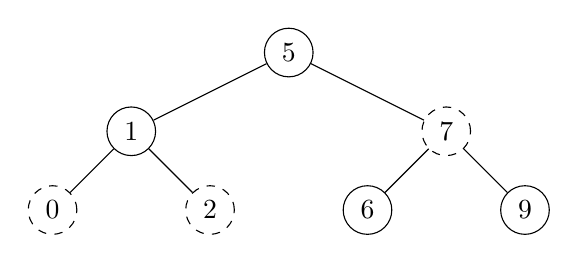
\begin{tikzpicture}
\node[shape=circle,draw=black] (5) at (0,0) {5};
\node[shape=circle,draw=black] (1) at (-2,-1) {1};
\node[shape=circle,draw=black,dashed] (0) at (-3,-2) {0};
\node[shape=circle,draw=black,dashed] (2) at (-1,-2) {2};
\node[shape=circle,draw=black,dashed] (7) at (2,-1) {7};
\node[shape=circle,draw=black] (6) at (1,-2) {6};
\node[shape=circle,draw=black] (9) at (3,-2) {9};

\path (5) edge (1);
\path (5) edge (7);
\path (1) edge (0);
\path (1) edge (2);
\path (7) edge (6);
\path (7) edge (9);
\end{tikzpicture}
\end{center}

\clearpage

{\bf Question 5 (20 Points)} \kern 0.5cm For the following hash functions, state
whether or not the function is ``good''.  Justify your answer.

\begin{enumerate}[label=(\alph*)]

\item Given any string of alpha-numeric characters, map all letters to integers
in the range $[0, 26)$ such that $a = 0$, $b = 1$, and so on.  Map all number
characters to their corresponding integer.  Take the index to be the sum of
this set of integers.  Assume this function is used in a hash table with
collision chaining.

\vspace{6cm}

\item Given an integer identifier $n$, create an index $i = \left \lfloor \frac{n}{10} \right \rfloor$.  Assume this function is used in a hash table with open addressing.

\end{enumerate}

\end{document}
